%%%%%%%%%%%%%%%%%%%%%%%%%%%%%%%%%
\section{Interfaces}
\label{sec:dp-tpcelec-intfc}

The \dword{dp} electronics system interfaces with several other systems, starting with the \dword{crp} and the \dword{pd} systems.  The digitized data must, in turn, flow to the \dword{daq} via the optical links in each \dword{utca} crate. The \dwords{sftchimney} integrate into the cryostat structure and connect to the cryogenics and gas systems. The slow-control system takes on management of the low-voltage power supplies for the \dword{fe} analog electronics and \dword{utca} crates and  monitors various sensors in the \dwords{sftchimney}. Table~\ref{tab:dp-tpcelec-interfaces} references the associated %relevant 
interface documents for each interface. %, stored in the DUNE document database (DocDB).

\begin{dunetable}
[TPC electronics system interface links]
{p{0.25\textwidth}p{0.5\textwidth}l}
{tab:dp-tpcelec-interfaces}
{TPC electronics system interface links}
Interfacing System & Description & Linked Reference \\ \toprowrule
\dword{crp} & signals from charge collection strips & \citedocdb{6751} \\ \colhline
\dword{pd} & signals from light detection sensors & \citedocdb{6772} \\ \colhline
\dword{daq} & transmission of digitized \dword{cro} and \dword{lro} data & \citedocdb{6778} \\ \colhline
\dword{cisc} & \dword{sftchimney} sensors, control of low-voltage power supplies for \dword{fe} cards, monitoring of \dword{utca} crates & \citedocdb{6784} \\ \colhline
Underground installation & transport of material and underground installation procedure & \citedocdb{7009} \\ \colhline
Integration facility  & logistics and use of integration facility & \citedocdb{7036} \\ \colhline
Calibration & calibration database format & \citedocdb{7063} \\ \colhline
DUNE physics & simulation of the electronics system & \citedocdb{7090} \\ \colhline
Software and computing & reconstruction and analysis tools for charge and light signals & \citedocdb{7117} \\ 
\end{dunetable}

%%%%%%%%%%%%%%%%%%%%%%%%%%%%%%%%%
\subsection{Electronics System to \dword{crp} and Photon Detection Systems}
\label{ssec:dp-tpcelec-intfc-crppmt}

The cold \fdth flange of the \dwords{sftchimney} forms the interface between the \dword{crp} and the \dword{cro} electronics system. On the side facing the cryostat, the flange \dword{pcb} has \num{20} \num{68}\, pin connectors (KEL 8930E-068-178MS-F\footnote{KEL Corporation\texttrademark{}, \url{https://www.kel.jp/english/product/product_detail/?id=490\&pageID=3\%20}.}) for plugging in the flat cables from the \dword{crp}. These flat cables are \num{68}\, channel twisted-pair cables, each carrying signals from \num{32} anode strips and within the scope of the \dword{crp} system. Each analog \dword{fe} card reads \num{64} anode strips, i.e., signals from two KEL connectors. The order in which the cables are connected to the cold flange determines the mapping of the electronic channels to the physical location of the strips on the \dword{crp} and is coordinated carefully with the \dword{crp} consortium. Figure~\ref{fig:dp-tpcelec-sft-cold-flange} shows two images of the cold \fdth from the \dword{wa105}.

\begin{dunefigure}[Images of the \dshort{wa105} \dshort{sft} cold \fdth]{fig:dp-tpcelec-sft-cold-flange}
{Images of the \dword{wa105} \dword{sft} cold \fdth with the \dword{fe} cards inserted (right) and signal cables from \dword{crp} connected (left). The \dword{wa105} \dwords{sftchimney} read only \num{320} channels and thus require \num{5} \dword{fe} cards. }%\fixme{to be updated with the ones from ProtoDUNE-DP after installation is finished}}
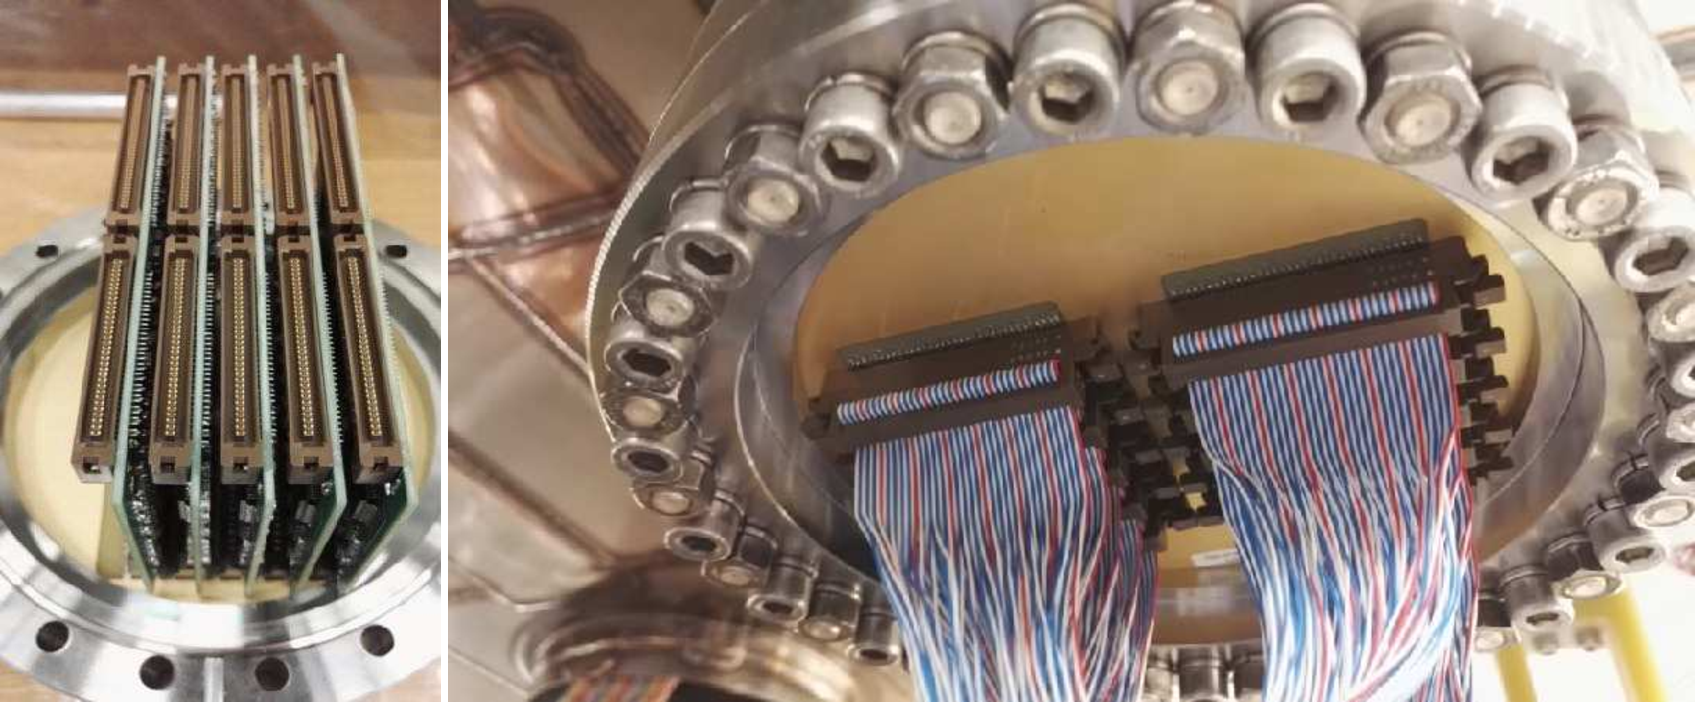
\includegraphics[width=0.8\textwidth]{dp-tpcelec-sft-cold-flange}
\end{dunefigure}

The \dword{lro} electronics system is connected to dedicated 
\dword{lro} signal \fdth flanges on top of the cryostat via coaxial cables provided by %, which are within the scope of the 
\dword{pds} consortium. 
%\fixme{The following does not seem to belong here. It's about gain and noise, not interfaces.} Since the electronics has to interface to PMTs whose signal polarity can be positive or negative depending on the base design and their gain can be also be varied, we think it is important to provide precise specifications here as to in what conditions the electronics system can work as designed
The \dword{lro} electronics is designed for negative polarity \dword{pmt} signals, with the amplitude of single \phel{}s on the input of the card between \num{1} and \SI{10}{\milli\volt}. Assuming a typical \dword{pmt} gain of \num{1e6} (not accounting for attenuation of the signals), the \dword{catiroc} \dword{asic} can measure a range of \num{1} to \num{400} \phel{}s (\SI{160}{\femto\coulomb} to \SI{70}{\pico\coulomb}). The \dword{adc} samples from \SI{1}{\milli\volt} to \SI{1}{\volt}, corresponding to \num{1} to \num{1000} \phel{}s; including the time response of the scintillator, the range can increase to approximately \num{6000}. Increasing the gain of the \dword{pmt} to \num{1E7}, reduces the upper values by a factor of 10. The internal noise level of the \dword{catiroc} is below \SI{0.1}{\milli\volt}. The objective for the noise level of the \dword{adc} is for each channel to have an \dword{rms} noise level higher than \SI{0.5}{LSB}, aiming for \SI{1}{LSB} \SI{0.1}{\milli\volt}.


%%%%%%%%%%%%%%%%%%%%%%%%%%%%%%%%%
\subsection{Electronics System to DAQ System}
\label{ssec:dp-tpcelec-intfc-daq}

%The \dword{dune} \dword{daq} is identical for \dword{spmod} and \dword{dpmod}. 
The \dword{dpmod} \dword{daq} is identical to the \dword{spmod} \dword{daq}. Although the architecture of the detector readout electronics is different for each technology, %between two technologies to adapt to the needs of the respective detector design, 
the output format of the generated data is the same, and both are synchronized to the same global clock signals. The readout data are continuously streamed via \SI{10}{Gbit/s} optical links 
by each \dword{detmodule} \dword{fe} electronics system to the \dword{daq}.  There they are aggregated and trigger primitives are constructed based on a common set of algorithms. A final trigger decision is then taken and, depending on the outcome, relevant data time slices are moved to a persistent storage. Figure~\ref{fig:dp-tpcelec-daq-interface-scheme} provides a schematic illustration of these concepts.
  
\begin{dunefigure}[Interface of \dshort{dp} \dshort{tpc} electronics to \dshort{daq}]{fig:dp-tpcelec-daq-interface-scheme}
{Schematic illustration of the interface of \dword{dp} \dword{tpc} electronics to \dword{daq}.}
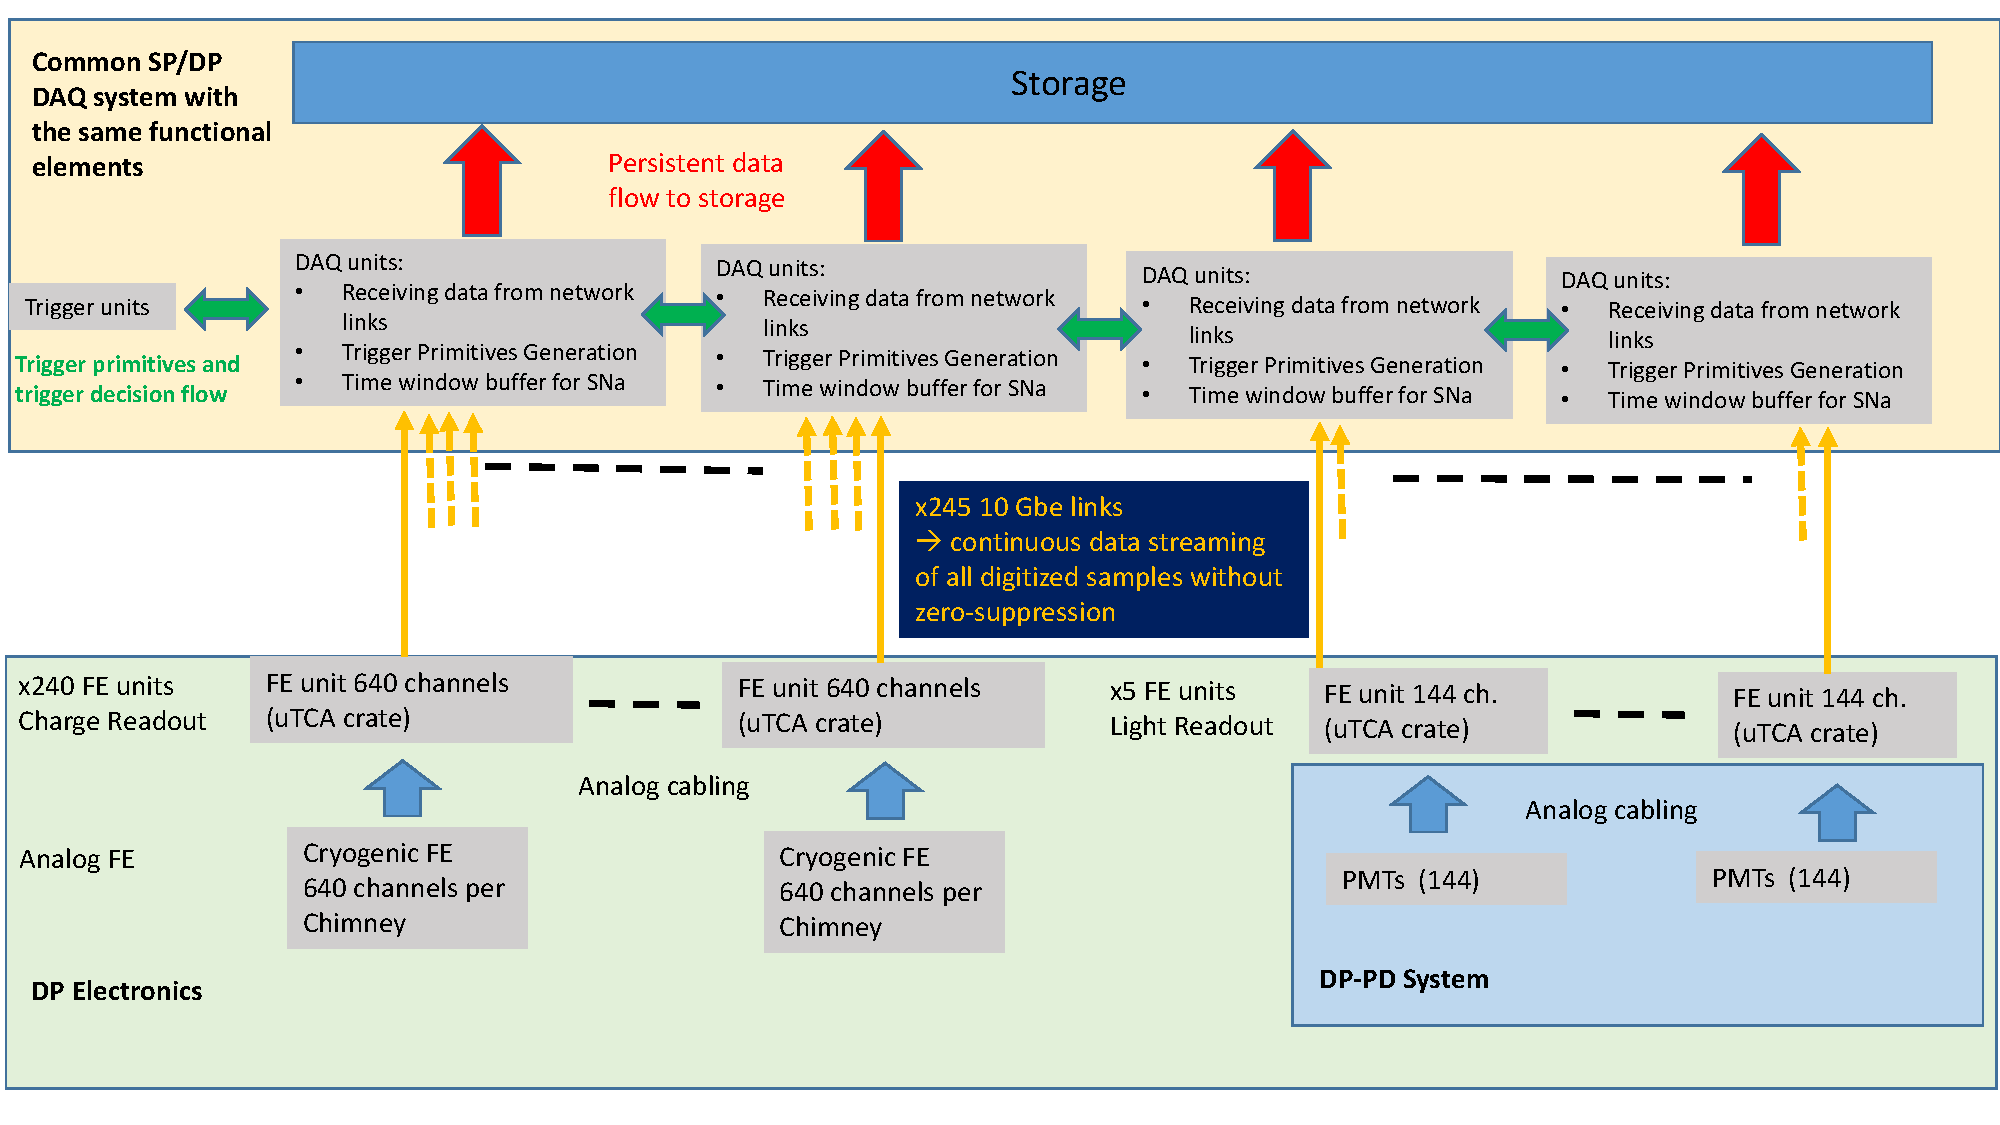
\includegraphics[width=0.95\textwidth]{dp-tpcelec-daq-interface-scheme}
\end{dunefigure}

The hardware interface between the \dword{dp} \dword{cro} and \dword{lro} electronics subsystems and \dword{daq} has two components. The first %interface uses 
is the \SI{10}{Gbit/s} optical fibers for data transfer between the \dword{utca} crates and the network interface of the \dword{daq} system. The second %interface 
is a \SI{1}{Gbit/s} optical fiber that connects the \dword{daq} \dword{wrgm} switch to the \dword{dp} electronics timing system.   


The \num{245} \SI{10}{Gbit/s} optical links stream the digitized data to the \dword{daq} from the \dword{cro} (\num{240} links) and \dword{lro} (\num{5} links) electronics housed in  the \dword{utca} crates on top of the cryostat.  The fibers, provided by the \dword{daq} consortium, are specified as multimode OM3 fibers \cite{om3fibers} with LC-LC connectors suitable for transmitting data over distances up to \SI{300}{\metre}.   On the side of the \dword{utca} crate, the fibers connect to an optical transceiver in the \dword{mch} (two SFP+XAUI links) \cite{natmch}.  On the \dword{daq}, they connect to the level-1 machines of the trigger farm or to switches, depending on the network topology adopted in the \dword{daq} system design.

The \SI{1}{Gbit/s} link going from the \dword{wrgm} to the \dword{dp} electronics time distribution network provides synchronization to the reference clock common %for 
to the entire \dword{fd} and derived from a GPSDO clock unit installed on the surface. The clock information is distributed to the \dword{wrmch} slave module in each \dword{utca} crate via a set of \dword{wr} switches. These switches and the interconnecting \SI{1}{Gbit/s} fibers form the timing subsystem of the \dword{dp} electronics system. % and are included in the design of that system. 
The \dword{wr} synchronization protocol includes the automatic and continuous calibration of the propagation delays between the master and the connected slaves. This allows maintenance of the  overall synchronization between different nodes at the sub-ns level. The \dword{wrgm} will be located in one of two places:
\begin{itemize}
\item{On the surface near the GPSDO. In this case, the system automatically accounts for the incurred latency due to the extensive length of a fiber that brings timing information underground.}
\item{Underground in the \dword{cuc}. In this case, propagation delays between GPSDO and the \dword{wrgm} are calibrated manually, and a timing correction is applied to the data afterward.}
\end{itemize} 



The software interface between the \dword{daq} and the electronics system includes tools for handling data transmission and buffering, i.e.,  data formatting in \dword{udp} packets, compression and decompression, and exchange of the control packets.

%%%%%%%%%%%%%%%%%%%%%%%%%%%%%%%%%
\subsection{Electronics System to Cryostat and Cryogenics}
\label{ssec:dp-tpcelec-intfc-cryo}

The interface points between the cryostat and the \dword{dp} electronics system %is %at 
are the cryostat penetrations, each of which % where the \dwords{sftchimney} are installed. Each penetration 
accommodates a %chimney 
\dwords{sftchimney} of external diameter \SI{254}{\mm}. Each chimney has a CF-273 flange welded to its outer structure (see Figure~\ref{fig:dp-tpcelec-sft-chimney-crosspipe}). After the chimney is inserted, this flange is in contact with the corresponding flange on the crossing (or penetration) pipe embedded in the cryostat structure to which it is eventually fastened. %To avoid any leaks at this interface a 
A CF-273 copper gasket is used to ensure vacuum tightness at this interface.  

%\fixme{Should be replaced with an image from the actual cryostat 3D model once the latter is ready}
\begin{dunefigure}[Details of \dshort{sftchimney} interface to the cryostat structure]{fig:dp-tpcelec-sft-chimney-crosspipe}
{Details of \dword{sftchimney} interface to the cryostat structure.}
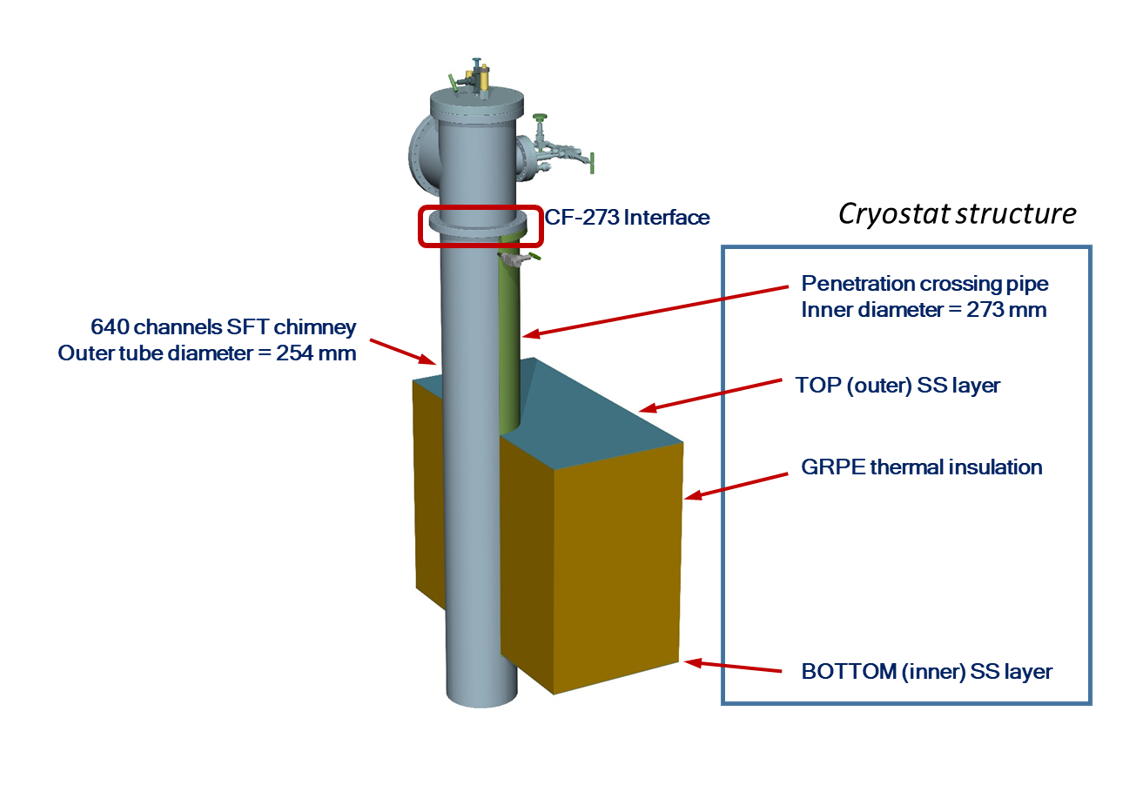
\includegraphics[width=0.7\textwidth]{dp-tpcelec-sft-chimney-crosspipe}
\end{dunefigure}

Each chimney contains a heat exchanger copper coil cooled with \dword{lar}. Two stainless steel pipe connections (inlet and outlet) with \SI{10}{\mm} (\SI{12}{\mm}) inner (outer) diameter must be branched: the inlet to the system for \dword{lar} delivery and the outlet to recirculation. In addition, a connection for a nitrogen gas line with the same pipe dimensions as for \dword{lar} cooling is used to fill the chimney after it is closed once the \dword{fe} electronics are installed. The nitrogen line is also required for flushing the chimney in case access is needed to the \dword{fe} cards after the \dword{dpmod} is cooled. % for the operation. 

The \dword{utca} crates for charge readout are installed within \SI{<0.5}{\meter} of the \dwords{sftchimney} on %top of 
the cryostat roof. The five \dword{utca} crates for light readout are also placed on the roof %of the cryostat 
at %optimal locations defined 
locations optimized for %by the routing of 
\dword{pmt} signal cable routing. The volume required  to accommodate the crates is roughly \SI[product-units=power]{60x50x40}{\cm}. 

%%%%%%%%%%%%%%%%%%%%%%%%%%%%%%%%%
\subsection{Electronics System to Slow Control System}
\label{ssec:dp-tpcelec-intfc-sc}

Integration with the slow control of the \dword{lv} power supply system for the \dword{fe} cards and \dword{utca} crates %is required to 
must enable remote management and monitoring. In addition, the \dwords{sftchimney} contain several sensors that require monitoring, e.g.,  %must be monitored. These include 
a pressure transducer that measures the pressure inside the chimney and at least two temperature probes (PT1000) that monitor the gas temperature inside the chimney, one near the cold flange at the bottom and one close to the warm flange at the top. The \dword{cisc} consortium is responsible for the readout of the \dword{utca} crate information and the sensors in the \dwords{sftchimney}. % is part of the slow control system.
